\section{Distribution Construction}

\subsection{Single Executable Distribution Construction}

In this method, the final goal is to have a set of distributions that can be compared to ground truth distributions to
determine whether or not the file contains malicious code.
Distributions are created by taking all the jumps between occurrences of a given op code, $op$, and aggregating it in
$b$ bins using the bin assignment function $\phi$ to discretize the data.
A jump is the number of instructions invoked between two opcodes of the same type.
Given the executable file has been converted to an opcode sequence, the indices of each opcode in the list can
be used to determine the jumps between successive op codes.
The construction of a single executable distribution set is shown in Algorithm \ref{alg:algorithm_single}.

\begin{center}
    $bin \; assignment:\; \phi(jump) = \lfloor \frac{jump}{1000} * bin_{size} \rfloor$
\end{center}

Since executables are of variable length, and it is possible for a jump to be close to the length of the entire
executable if occurrences are sparse, jump values are capped at 1000 to reduce extreme outliers.
These large jumps are infrequent, so keeping them would skew the distributions and subsequent comparisons to
such distributions.
Any jump value whose bin assignment falls outside the number of bins is omitted.

%! Author = jacobcarlson
%! Date = 4/26/23

\begin{algorithm}
    \caption{Single Executable Distribution Algorithm}
    \begin{algorithmic}
%        \STATE  $\mathrm{train\_ANN} (f_i,w_i,o_j)$
        \FOR{$op$ in opcode set}
            \STATE $N_{op} \gets $ number of op occurrences
            \STATE $distribution_{op} \gets 0$ vector the size of the number of bins
            \FOR{each occurrence of $op$ in sequence = $1$ to $(N_{op}-1)$}
                \STATE $jump_{op\_k} = op_{k+1} - op_{k}$
                \STATE $distribution_{op}[\;\phi(jump_{op\_k})\;]$ += 1
            \ENDFOR
            \FOR{each bin $b$ in $distribution_{op}$ = $1$ to $B$}
                \STATE $distribution_{op}[b]$ \textbackslash= $(N_{op}-1)$
            \ENDFOR
        \ENDFOR
    \end{algorithmic}\label{alg:algorithm_single}
\end{algorithm}

\subsection{Multiple Executable Distribution Construction}
The process to create aggregated distributions is similar to the algorithm for individual files, with the exception that
the distribution is aggregated over a large number of files of the same class.
By only aggregating files over one class, distribution sets are created that are representative of what a typical
jump distribution from a single executable should look like.
The construction of a multiple executable distribution set is shown in Algorithm \ref{alg:algorithm_multiple}.

The values obtained from comparing a code sample to a ground truth distribution of each class over all opcodes in
an opcode set will generate a vector of values twice the size of the opcode set, each distribution is compared to a
benign and malicious ground truth.
This will be used as the input to machine learning models for each sample.

%! Author = jacobcarlson
%! Date = 4/26/23

\begin{algorithm}
    \caption{Multiple Executable Distribution Algorithm}
    \begin{algorithmic}
        \FOR{$op$ in opcode set}
            \STATE $distribution_{op} \gets 0$ vector the size of the number of bins
        \ENDFOR
        \FOR{executable $l$ = $1$ to $L$}
            \FOR{$op$ in opcode set}
                \STATE $N_{l\_op} \gets $ number of op occurrences in $l$
                \FOR{each occurrence of $op$ in sequence = $1$ to $(N_{l\_op} - 1)$}
                    \STATE $jump_{l\_op\_k} = op_{l\_k+1} - op_{l_k}$
                    \STATE $distribution_{op}[\;\phi(jump_{l\_op\_k})\;]$ += $1$
                \ENDFOR
            \ENDFOR
        \ENDFOR
        \FOR{$op$ in opcode set}
            \STATE $total\_jumps_{op} \gets \sum_{b=1}^B distribution_{op}[b]$
            \FOR{each bin $b$ in $distribution_{op}$ = $1$ to $B$}
                \STATE $distribution_{op}[b]$ \textbackslash= $total\_jumps_{op}$
            \ENDFOR
        \ENDFOR
    \end{algorithmic}\label{alg:algorithm_multiple}
\end{algorithm}

Ten ground truth samples were created for each class, each sample is aggregated over 500 total files and no file was in
used in multiple ground truth distributions.
To show that there was some form of similarity between distributions of the same class, heatmaps were created to
show comparisons between all ground truth samples.
Each cell displays the sum of the Kullback-Leibler divergence between two ground truth sets over all the
distributions in the set.
This does not completely prove that the distributions are similar, but if the value of the sum is low, then that
should show that the set of distributions are more similar than if the value is high.

Figure \ref{fig:example_heatmaps} shows heatmap examples of two different opcode sets.
Both examples show two distinct sets of low KL Divergence, one grouping of benign ground truth distributions
and another grouping of malicious ground truth sets.

\begin{figure}[H]
    \centering
    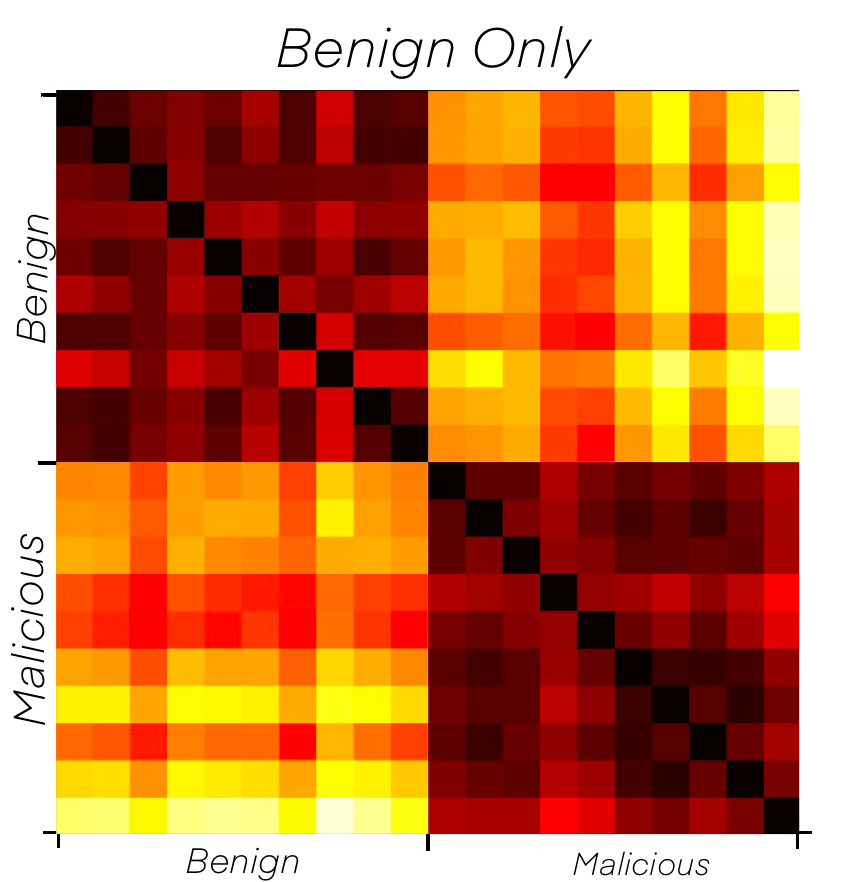
\includegraphics[width=0.2\textwidth]{jump_benign}\hspace{1em}%
    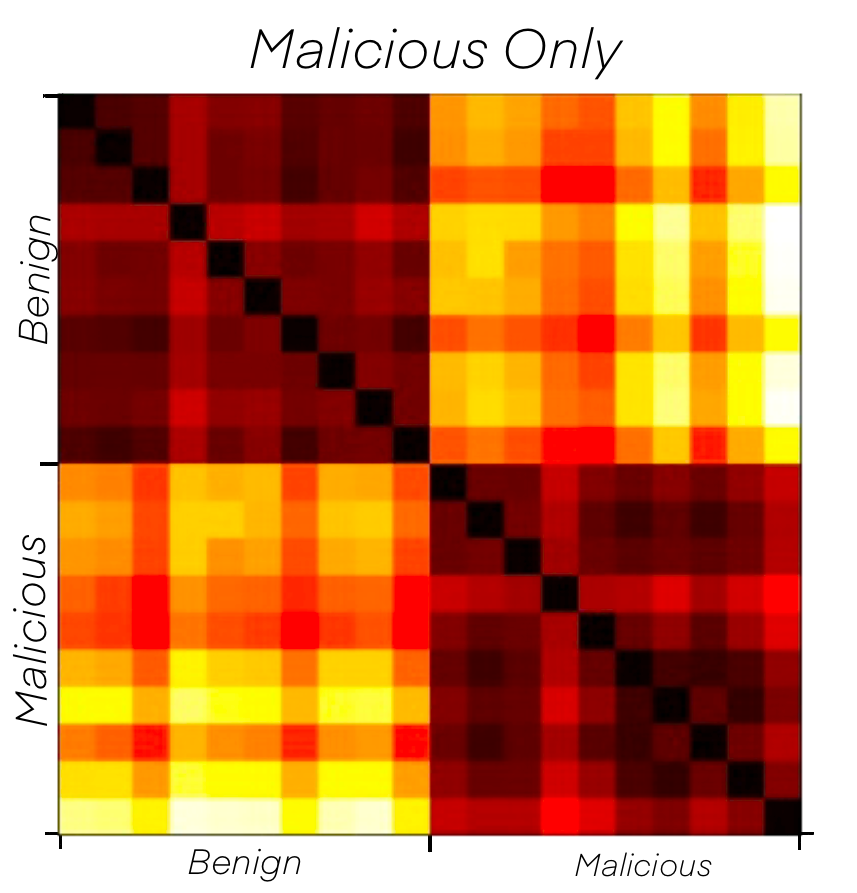
\includegraphics[width=0.2\textwidth]{jump_malicious}
    \centering
    \caption{
        Benign and Malicious Heatmaps
    }
%    \footnotesize{Heatmaps for 20 ground truth samples, 10 of each class. Cells of a darker color indicated lower
%        Kullback-Leibler Divergence values, while cells of a lighter color indicate higher KL Divergence values.}
    \label{fig:example_heatmaps}
\end{figure}

